%Projekt 5 - FILIP JEŽOVICA - xjezov01
\documentclass{beamer}
\usetheme{Berlin}

\usepackage[czech]{babel}
\usepackage[utf8]{inputenc}
%\usepackage[T1]{fontenc}
\usepackage{picture}
\usepackage{graphics}


\begin{document}

\title{Systém \LaTeX}
\subtitle{Úvod do vsádzacieho systému \LaTeX}
\author{Filip Ježovica \\
		xjezov01@stud.fit.vutbr.cz}
\institute{Vysoké učení technické v~Brně\\Fakulta informačních technologií}


\frame{\titlepage} 

\frame{\frametitle{Úvod}
\begin{itemize}
\item \LaTeX je typografický systém
\item vyvinutý v~roku 1985 Lesliem Lamportom
\item vhodný na vytváranie rôznych typov dokumentov
\item \LaTeX je voľne dostupný - zdarma
\item podobný programovaciemu jazyku
\item môžeme ho používať na rôznch systémoch
\end{itemize} 
}

\frame{\frametitle{Kde ho môžeme používať?}
Systém \LaTeX je možné používať na týchto systémoch:
\begin{itemize}
\item Windows
\item Linux
\item Mac OS
\item UNIX
\item \dots
\end{itemize} 
}

\frame{\frametitle{Grafické rozhranie}
Dokument môžme napísať v~akomkoľvek textovom editore.
Následne je nutné ho preložiť \LaTeX ovým prekladačom.
Existujú i~grafické rozhrania pre uľahčenie práce.

\begin{figure}[h]
\begin{center}
    \scalebox{0.2}{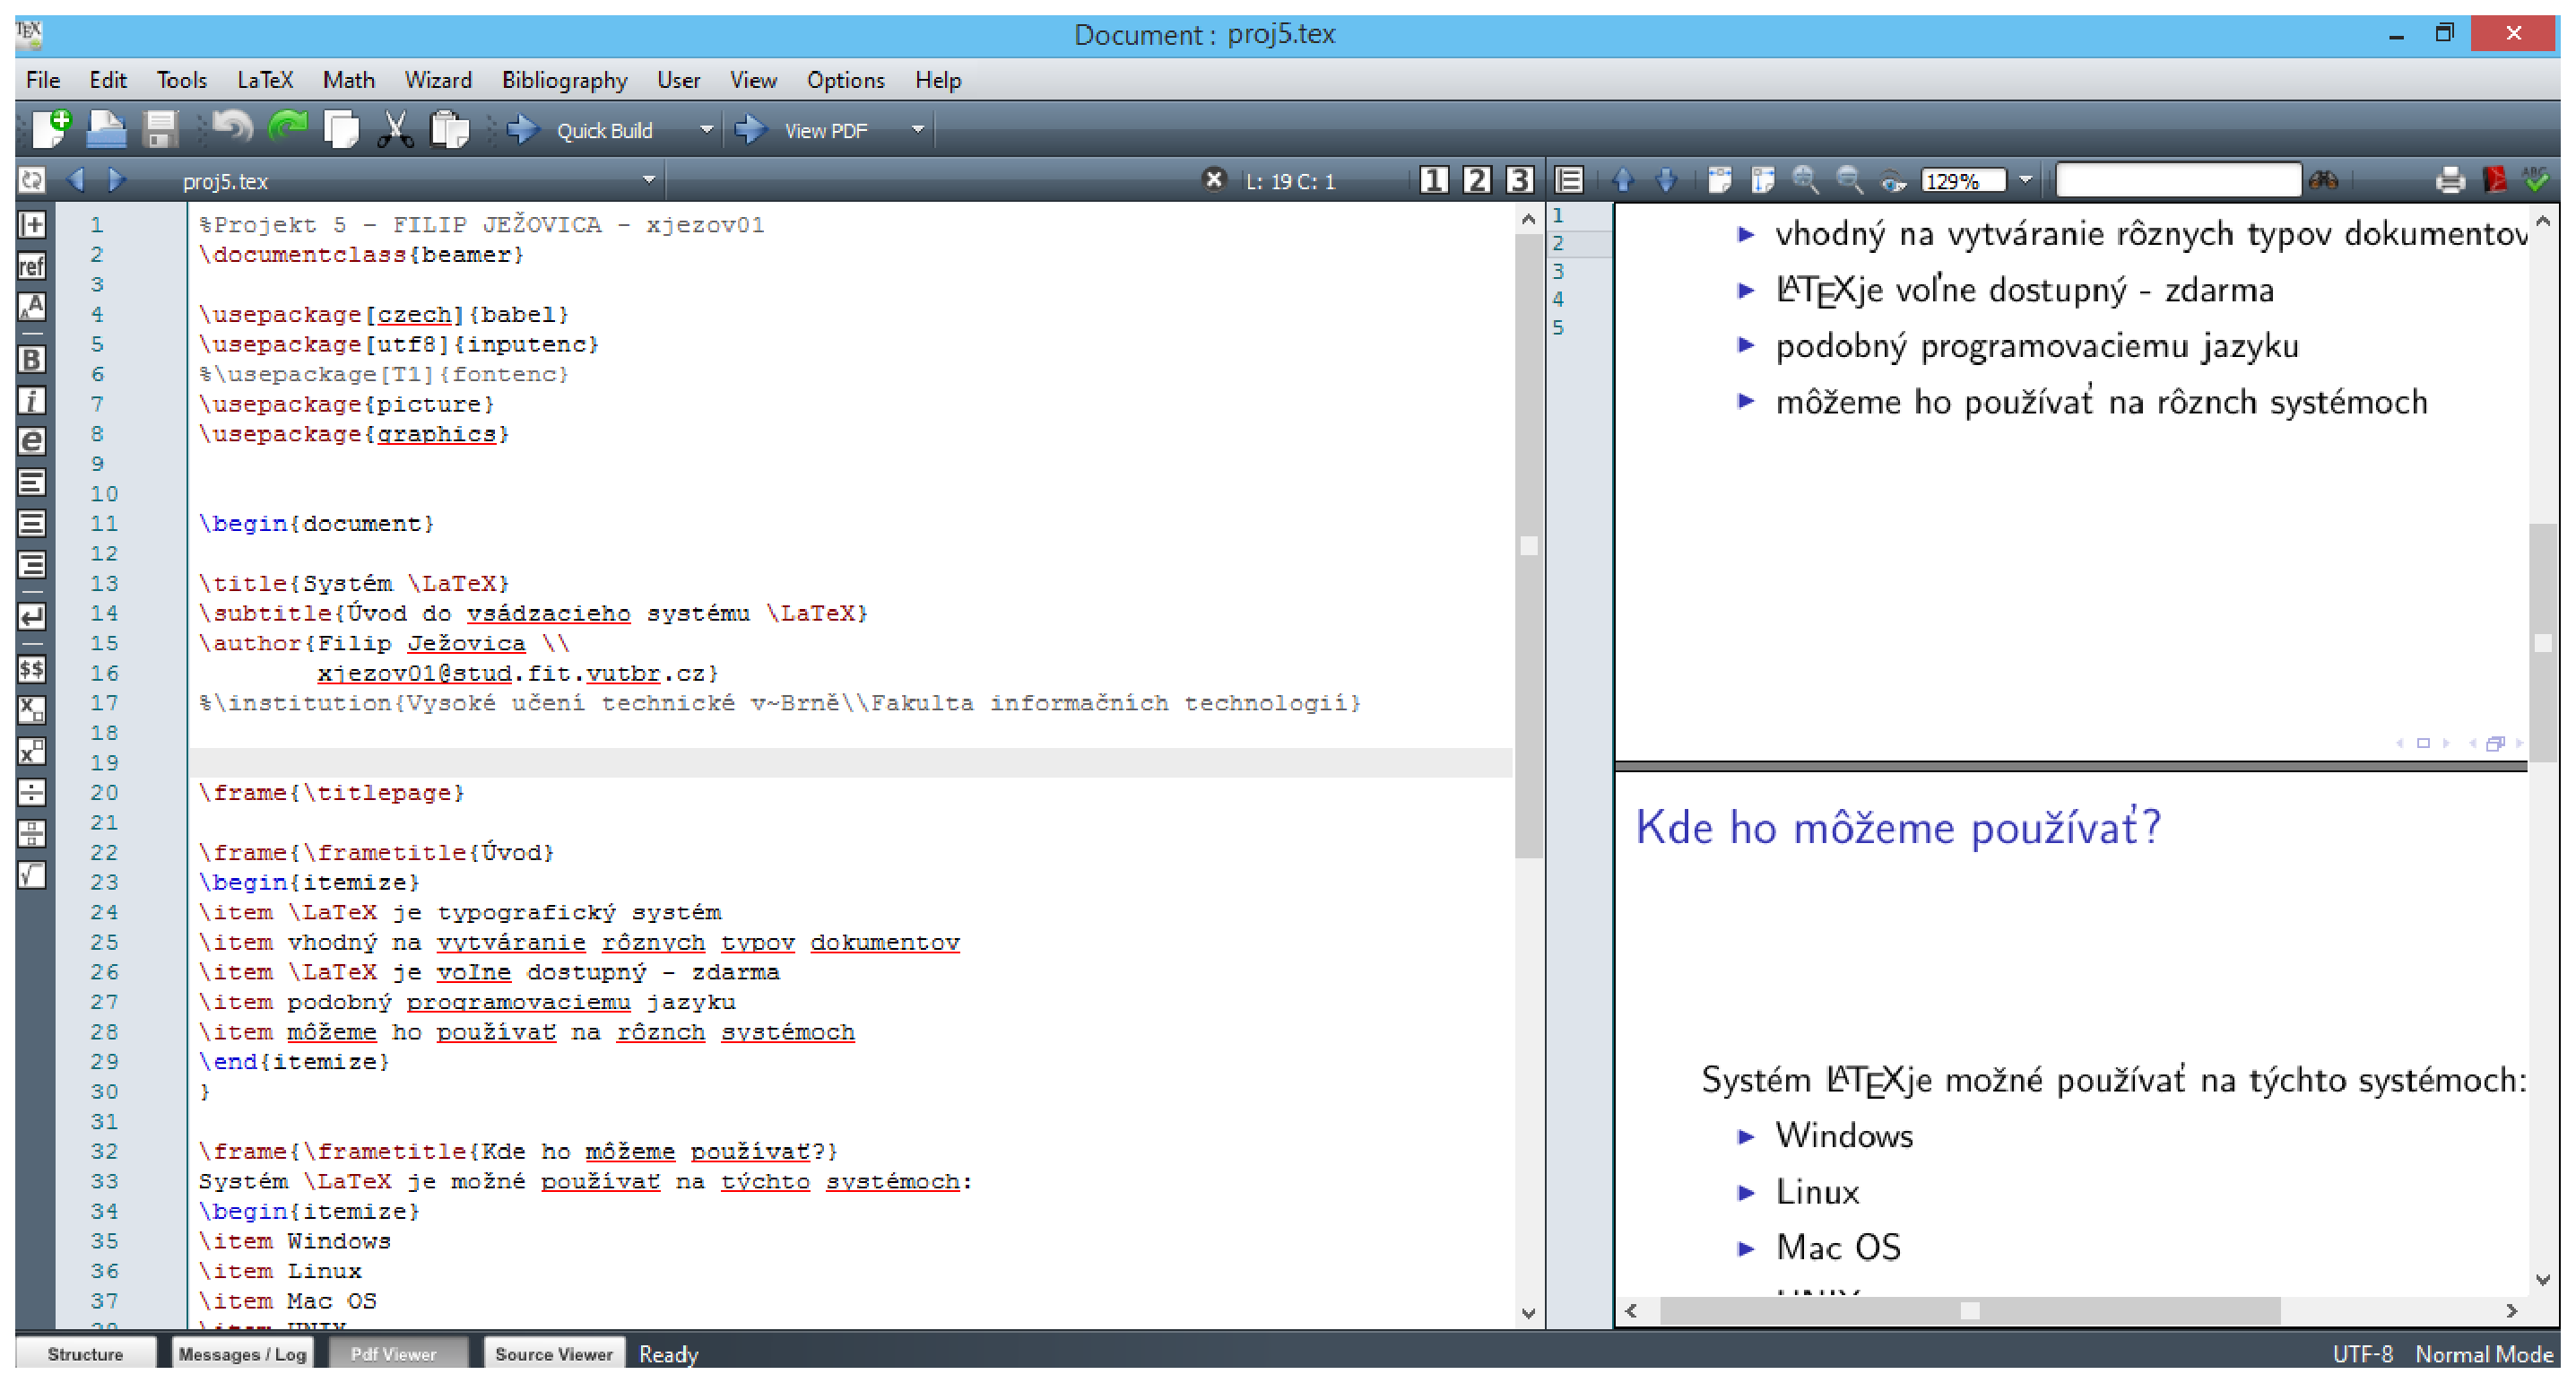
\includegraphics{screenshot.eps}}
    \caption{Ukážka grafického rozhrania \TeX maker} \label{obrazok:screenshot}
\end{center}
\end{figure}
}

\frame{\frametitle{Grafické rozhranie}
Poznáme tieto grafické rozhrania, ktoré poznajú syntax \LaTeX u:
\begin{itemize}
\item \TeX maker \pause
\item WinEdt \pause
\item \TeX works \pause
\item LEd \pause
\item Sublime
\item \dots
\end{itemize} 
}

\frame{\frametitle{\LaTeX om vyhradené špeciálne znaky}
Ak tieto znaky použijeme v~zdrojovom súbore tak sa na výstupe nezobrazia - majú špeciálny význam.

Ak chceme aby tieto znaky boli viditeľné vo výstupnom súbore, je potrebné pred ne dať znak \textbackslash \\

Sú to tieto znaky:
\begin{tabular}{p{0.4\textwidth}p{0.5\textwidth}}

\begin{itemize}
     \item \textbackslash
     \item \#
     \item \{
     \item \}
     \item \_
  \end{itemize} &

\begin{itemize}
	\item \$
	\item \%
	\item \&
	\item \textasciicircum
	\item \textasciitilde
\end{itemize} \\

\end{tabular}

}

\frame{\frametitle{Použitá literatúra}
\begin{itemize}
\item J. Rybička. LATEX pro začátečníky. Konvoj, Brno, 1995
\item https://www.cstug.cz/
\end{itemize}
}

\frame{
\begin{center}
{\LARGE Ďakujem za pozornosť}
\end{center}
}


\end{document}